\documentclass[article]{jss}
%\usepackage[T1]{fontenc}
%\usepackage[latin9]{inputenc}
%\usepackage{url}
%\usepackage{graphicx}
%\usepackage[authoryear]{natbib}
%\usepackage{babel}
%\usepackage{fullpage}
%\usepackage{hyperref}
%\newcommand{\pkg}[1]{{\fontseries{b}\selectfont #1}}

%%%%%%%%%%%%%%%%%%%%%%%%%%%%%%
%% declarations for jss.cls %%%%%%%%%%%%%%%%%%%%%%%%%%%%%%%%%%%%%%%%%%
%%%%%%%%%%%%%%%%%%%%%%%%%%%%%%

%% almost as usual
\author{Xiaoyue Cheng\\Iowa State University \And 
        Dianne Cook\\Iowa State University \And
        Heike Hofmann\\Iowa State University}
\title{Visually Exploring Missing Values in Multivariable Data 
       Using a Graphical User Interface}

%% for pretty printing and a nice hypersummary also set:
\Plainauthor{Xiaoyue Cheng, Dianne Cook, Heike Hofmann} %% comma-separated
\Plaintitle{Visually Exploring Missing Values in Multivariable Data 
	    Using a Graphical User Interface} %% without formatting
\Shorttitle{Visually Exploring Missing Values} %% a short title (if necessary)

%% an abstract and keywords
\Abstract{
  Missing values are common in data, and usually require attention in order to conduct the statistical analysis.  One of the first steps is to explore the structure of the missing values, and how missingness relates to the other collected variables.  This article describes an \proglang{R} package, that provides a graphical user interface (GUI) designed to help explore the missing data structure and to examine the results of different imputation methods. The GUI provides numerical and graphical summaries conditional on missingness, and includes  imputations using fixed values, multiple imputations and nearest neighbors.
}
\Keywords{missing values, imputation, exploratory data analysis, 
	  statistical graphics, data visualization, graphical user interface}
\Plainkeywords{missing values, imputation, exploratory data analysis, 
	statistical graphics, visualization, graphical user interface}

%% publication information
%% NOTE: Typically, this can be left commented and will be filled out by the technical editor
%% \Volume{50}
%% \Issue{9}
%% \Month{June}
%% \Year{2012}
%% \Submitdate{2012-06-04}
%% \Acceptdate{2012-06-04}

%% The address of (at least) one author should be given
%% in the following format:
\Address{
  Xiaoyue Cheng\\
  Department of Statistics and Statistical Laboratory\\
  Iowa State University\\
  2406 Snedecor Hall\\
  Ames, IA, 50011, United States of America\\
  E-mail: \email{xycheng@iastate.edu}\\
  URL: \url{http://xycheng.public.iastate.edu/}\\
  \\
  Dianne Cook\\
  Department of Statistics and Statistical Laboratory\\
  Iowa State University\\
  2415 Snedecor Hall\\
  Ames, IA, 50011, United States of America\\
  E-mail: \email{dicook@iastate.edu}\\
  URL: \url{http://dicook.public.iastate.edu/}\\
  \\
  Heike Hofmann\\
  Department of Statistics and Statistical Laboratory\\
  Iowa State University\\
  2413 Snedecor Hall\\
  Ames, IA, 50011, United States of America\\
  E-mail: \email{hofmann@iastate.edu}\\
  URL: \url{http://hofmann.public.iastate.edu/}\\
}
%% It is also possible to add a telephone and fax number
%% before the e-mail in the following format:
%% Telephone: +43/512/507-7103
%% Fax: +43/512/507-2851

%% for those who use Sweave please include the following line (with % symbols):
%% need no \usepackage{Sweave.sty}

%% end of declarations %%%%%%%%%%%%%%%%%%%%%%%%%%%%%%%%%%%%%%%%%%%%%%%


\begin{document}

\section{Introduction}\label{introduction}

Missing values are a very common problem affecting data analysis. Many imputation methods have been developed but little has been done for exploring the missing value structure visually.  Most plotting methods handle missing values by simply removing the incomplete records with or without a warning, especially when the data are continuous. Most statistical functions provide a limited list of handling missing values, such as, delete all cases with any missing values, delete pairwise or on single variables only.

The issue is, that in order to decide what to do with the missing values before analyzing the data, we need to understand what the distribution of the missing values is, and how the missingness depends on the other collected variables. A few \proglang{R} packages, like \pkg{Hmisc} \citep{hmisc}, \pkg{norm} \citep{norm}, and \pkg{mice} \citep{mice}, have some routines for summarizing the number of missing by variable, and by case, in preparation for imputing the missing values. To understand the distribution of missings versus non-missings it is also important to make plots of the data.

For model-based imputation methods, it is important to check assumptions like missing completely at random (MCAR) or missing at random (MAR). These are not easy to verify. \citet{little1988test} provided tests of the MCAR assumption, under normality conditions, and \citet{jaeger2006testing} proposed a test for MAR under some distributional conditions. Both tests employ inference based on likelihood ratios, and caution that the tests are sensitive to model misspecification \citep{little1988test}.  Visual exploration of the missingness can help check the assumptions: it cannot prove any randomness assumption holds but visual checks can be used to reject MCAR or MAR assumptions. Visual exploration can suggest what dependencies exist, and should be incorporated into imputation for MAR data.

Some existing work describing visual exploration of missingness, and implementations, can be found in \citet{unwin1996interactive}, \citet{swayne1998missing}, and \citet{templ2008visualization}. \proglang{MANET} \citep{unwin1996interactive} implements the interactive methods to missing data. It presents the segmented barcharts of missing versus non-missing values for each variable, and with its many plot types like histograms, scatterplots, and mosaic plots, encourages the user to select cases that are missing on any variable to highlight in other plots. This enables the user to explore the missing status dependence in the distributions of the complete cases of other variables. \proglang{XGobi} \citep{swayne1998xgobi}, which implements the ideas described in \citet{swayne1998missing}, is similar to MANET, but focuses on interactive graphics for exploring missing values in real-valued data. It creates a shadow matrix of the original data where entries are 0 (complete) or 1 (missing value). This additional data structure allows the user to explore the multivariate pattern of missing values, the dependence between missing value status and complete cases, and compare imputation mehtods. These ideas were re-implemented in \proglang{GGobi} \citep{STLBC03}.

In the \proglang{R} community, the package \pkg{VIM} \citep{VIM} provides a graphical user interface via \pkg{VIMGUI} \citep{VIMGUI}, to explore the structure of missing values and the quality of several single imputation methods (kNN, hotdeck, irmi). Some packages for multiple imputation have interfaces for easy manipulation, for example, \pkg{migui}, \code{AmeliaView()} and \pkg{miP}. The \pkg{migui} \citep{migui} is an interface for \pkg{mi} \citep{mi}, which implements multiple imputation via Bayesian models and weakly informative prior distributions. The function \code{AmeliaView()} in \pkg{Amelia} \citep{amelia}, generates a graphical interface, to implement its ``EM with bootstrapping'' algorithm. The package \pkg{miP} \citep{mip} adopts \pkg{VIM} to visualize the imputation results from packages \pkg{mice}, \pkg{mi}, and \pkg{Amelia}.

This current work describes a new package for \proglang{R}, \pkg{MissingDataGUI}, which allows the exploration of missing value structure, and comparison of different imputations, using static graphics and numerical summaries. The GUI makes these methods accessible for novice users. This work builds on the ideas developed in \citet{unwin1996interactive} and \citet{swayne1998missing}. The package utilizes routines in \pkg{Hmisc}, \pkg{norm}, \pkg{mice}, and \pkg{mi} for multiple imputation, and provides several other routines including kNN, random sampling and fixed values for the single imputation. Section \ref{Functionality} explains the GUI design, functionality and rationale.  Section \ref{Examples} gives a usage example. 


\begin{center}
\begin{figure}[h]
\begin{centering}
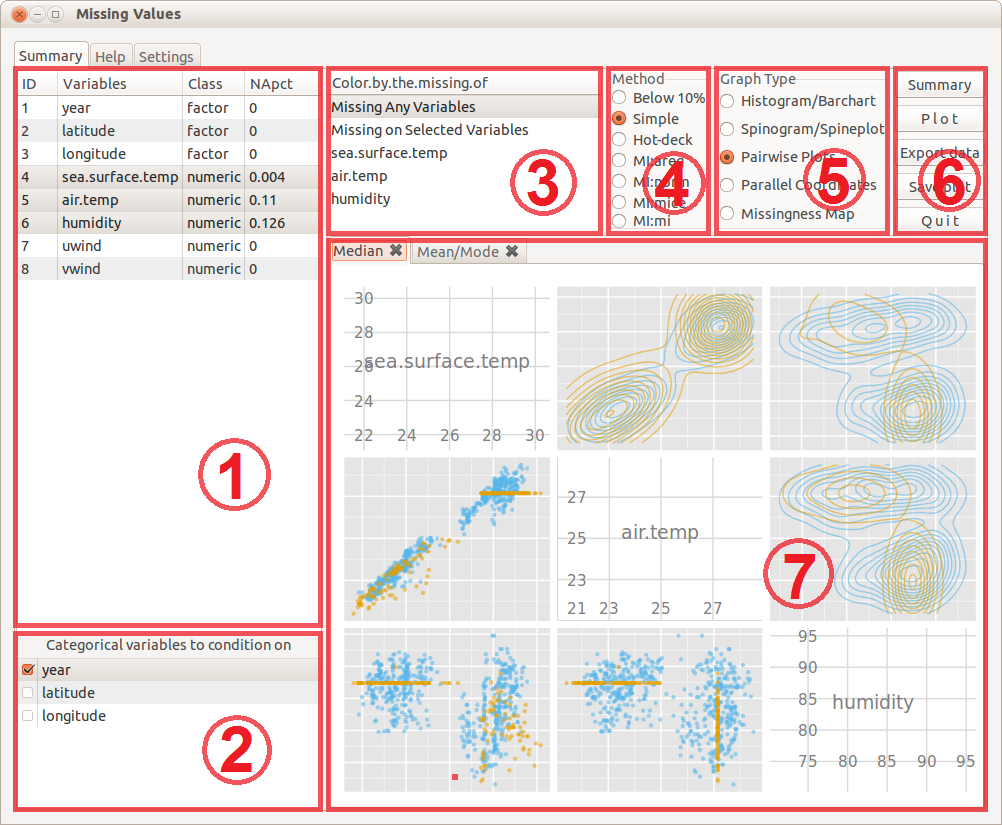
\includegraphics[width=.9\textwidth]{graph/fig1-GUI-tab1}
\par\end{centering}
\caption{Overview of the missing data GUI. Region 1 contains the list of variables, variable type, and summary of missings on that variable. Region 2 has a list of the categorical variables that can be used for conditioning plots and imputations. Region 3 has a selection panel for selection of coloring by different types of missingness in the plots. Region 4 contains a radio button selection of imputation methods. Region 5 has several plot type selections, and region 6 allows selecting numeric or graphical summaries and some output routines. The summaries are displayed in the region 7.}
\label{fig:missingGUI}
\end{figure}
\par\end{center}

\section{Functionality}\label{Functionality}

\subsection{Overview of the missing data GUI}

The appearance of the missing data GUI is shown in Figure~\ref{fig:missingGUI}. (Section \ref{Examples} describes the dataset.) All variables in the data along with the variable type and the percentages of \code{NA}'s are listed on the top left (region 1). The categorical variables (factor, ordinal factor, and character), auto-detected by their type, are shown on the bottom left as the potential conditioning variables (region 2). The variables having missing values are displayed under ``Color.by.the.missing.of'' on the top center (region 3). The graphical summary will distinguish the imputations from the observations by two colors, yellow (missing) versus blue (not missing). This panel is used to choose what missing structure to color. Selecting the first row ``Missing Any Variables'' means that the color will depend on whether the case has missing values in any variables. The second row ``Missing on Selected Variables'' means the graph is colored by whether the case has missings in the selected variable. ``Method'' (region 4) and ``Graph Type'' (region 5) are two widgets illustrated in Sections \ref{imputation} and \ref{plottype}. On the top right (region 6) there are five buttons: ``Summary'' can create a window as described in Section \ref{numsum}; ``Plot'' produces the plots in the graphics panel on the bottom right of GUI (region 7); ``Export data'' saves the imputed data into a file or to an \proglang{R} data frame; ``Save plot'' saves the plots in region 7 to png files; ``Quit'' destroys the main GUI window and the derived child windows.

\subsection{Summary of missing values}\label{numsum}

\subsubsection{Numerical summaries}
To investigate missingness in a data set, start examining the numerical summaries of the missings. The ``Summary'' button will open a window with the overall missingness information (Figure~\ref{fig: num-summry} left panel) or conditional summary (Figure~\ref{fig: num-summry} right panel), depending on whether conditioning variables are chosen. Both summary windows present the percent of the values that are missing, the percent of variables that contain missing values, the percent of the cases that have at least one missing value, along with a tabulation of the number of values missing per case. The style of the table follows the summary provided by the package \pkg{norm}.  In Figure~\ref{fig: num-summry} (left) it can be seen that the data has two observations have 3 missing values, another two have 2 missing values, 167 observations have one missing value and 565 are complete. By percentages, 76.8\% of the cases have no missings. Figure~\ref{fig: num-summry} (right) is conditioned on the variable ``year'', which produced two boxes for 1993 and 1997 respectively. We can see that there are fewer missing values in 1997 than 1993, and all the observations having more than 1 missings appeared in 1993.

\begin{center}
\begin{figure}[h]
\begin{centering}
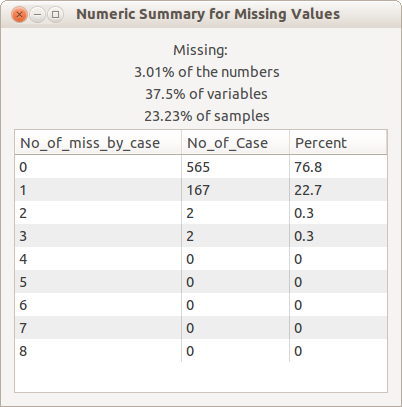
\includegraphics[width=0.33\textwidth]{graph/fig2-summary-1}
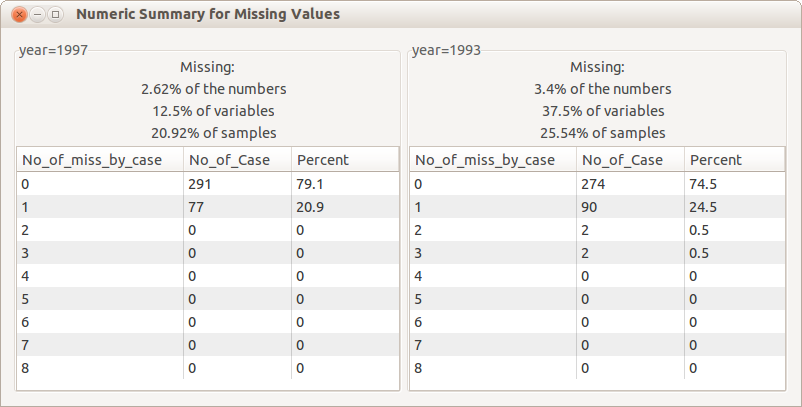
\includegraphics[width=0.66\textwidth]{graph/fig2-summary-2-condition}
\par\end{centering}
\caption{A numerical summary of missing values in the data is shown in a pop-up window. The left panel is the overall summary. The right panel shows the summary conditioned on ``year''. The percentages of missings by total number of data values, by variables and by cases, is shown on the top. This dataset has 8 variables and the missing values by variable are summarized in the bottom table. No cases have more than 3 missing values,  76.8\% of cases are complete, 22.7\% of cases have one missing value, and only 4 cases have more than one missing values. The right panel shows that the missing pattern is different for each year.}
\label{fig: num-summry}
\end{figure}
\par\end{center}

\subsubsection{Missingness map}

The missingness map (Figure~\ref{fig:missingmap}) provides a graphical summary of the missing patterns. Like the shadow matrix used in \proglang{GGobi}, the missingness map shows the position of missing values relative to variables and cases. The \proglang{R} package \pkg{Amelia} \citep{amelia}, and \pkg{VIM} \citep{VIM} have versions of missingness maps. Agglomerating the missing values into blocks by re-ordering variables and case ids, can enhance the understanding of missing patterns, especially for large data. Two re-ordered missingness maps are shown in Figure~\ref{fig:missingmap}. One arranges the variables and cases by the number of missings, from the largest to the smallest; the other applies hierarchical clustering to both rows and columns. The strength of missingness map is to reveal whether the missings occur at some variables simultaneously. If so, then a similar missing pattern may indicate some association between the variables. If the missings happen at some observations synchronously, then it suggests the dependence between those observations.

Figure~\ref{fig:missingmap} displays 245 observations and 34 variables for the dataset \code{brfss} (described in Section~\ref{Examples}). From the missingness maps we can see that most of the missings occurred in seven variables. The missingness of some variables are associated, and users should check the data collection procedure for these variables. In this example, the questions about the drinking time and amount (ALCDAY4 and AVEDRNK2, the top two variables in the right panel) were both skipped under the condition that the subject did not drink in the past 30 days. For those variables, the imputed values are of no interest. Instead, looking for the covariates of the condition is meaningful, so the plots colored by the missingness of ALCDAY4 and AVEDRNK2 will help.

\begin{center}
\begin{figure}[h]
\begin{centering}
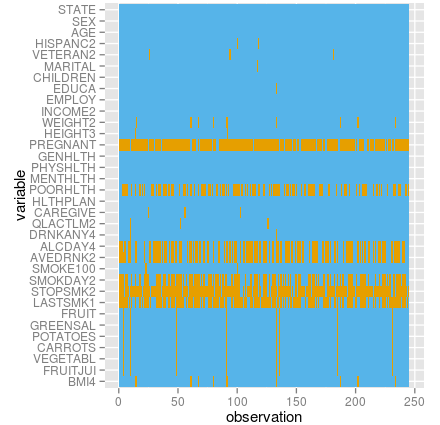
\includegraphics[width=0.3\textwidth]{graph/fig5-3-missingmap-1}
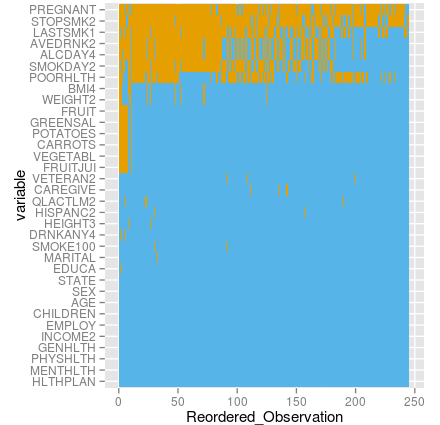
\includegraphics[width=0.3\textwidth]{graph/fig5-3-missingmap-2}
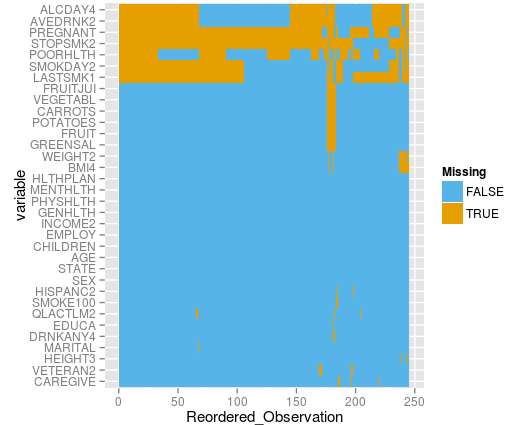
\includegraphics[width=0.345\textwidth]{graph/fig5-3-missingmap-3}
\par\end{centering}
\caption{Missingness maps with different orders of variables and cases. The left panel gives the original order; the middle one sorts the variables and cases by a decreasing number of missing values; the right one sorts them by a hierarchical clustering of missingness. From the original missingness map we see some variables with high missing rate, and several vertical segments at the bottom. In the middle panel the yellow color is clustered, although still messy, we can see some relationship between missing variables and observations. From the clustered missingness map on the right, we find that the missingness on the top two variables are strongly associated.}
\label{fig:missingmap}
\end{figure}
\par\end{center}

\subsection{Imputation}\label{imputation}

A number of imputation methods are available in the package. The purpose of these is not only to examine the dependence between missings or non-missings, but also to produce a complete data set for later analysis. A few criteria were considered to improve the user experience: (1) easy to understand and implement; (2) computing complexity is medium or low; (3) adaptability to different situations, i.e., no strong model assumptions. Not all of the imputation methods are available in the package, because (1) there are too many methods and variations, it is not practical to include all; and (2) users may use their own method and import the result to missing data GUI for exploration.

The seven imputation methods provided are: 
``Below 10\%'', ``Simple'', ``Neighbor'', ``MI:areg'', ``MI:norm'', ``MI:mice'', ``MI:mi''. 
``Simple'' and ``Neighbor'' contain more than one method. As shown in Figure~\ref{fig:missingGUI}, region 7, the three tab labels interface to the three methods provided by ``Simple'': overall median, mean/mode, and random value. ``Neighbor'' contains two methods: mean of the nearest neighbors, and random nearest neighbor. The neighbor methods also allow the user to change the number of neighbors. Table~\ref{tab:compare-methods} compares the imputation methods available in the GUI.

\begin{center}
\begin{table}[h]
\begin{centering}
\begin{tabular}{l|l|c|c|c}
\hline 
\textbf{\scriptsize{Method}} & \textbf{\scriptsize{Description}} & \textbf{\scriptsize{Determinisitic}} & \textbf{\scriptsize{Univariate}} & \textbf{\scriptsize{Multiple imp.}}\tabularnewline
\hline 
{\scriptsize{Below 10\%}} & {\scriptsize{below 10\% of the range}} & {\scriptsize{x}} & {\scriptsize{x}} & \tabularnewline
\hline 
 & {\scriptsize{overall median}} & {\scriptsize{x}} & {\scriptsize{x}} & \tabularnewline
{\scriptsize{Simple}} & {\scriptsize{overall mean/mode}} & {\scriptsize{x}} & {\scriptsize{x}} & \tabularnewline 
 & {\scriptsize{random value}} &  & {\scriptsize{x}} & \tabularnewline
\hline
{\scriptsize{Neighbor}} & {\scriptsize{mean of the nearest neighbors}} & {\scriptsize{x}} &  & \tabularnewline
 & {\scriptsize{random nearest neighbor}} &  &  & \tabularnewline
\hline 
{\scriptsize{MI:areg}} & {\scriptsize{predictive mean matching}} &  &  & {\scriptsize{x}}\tabularnewline
\hline 
{\scriptsize{MI:norm}} & {\scriptsize{multivariate normal model}} &  &  & {\scriptsize{x}}\tabularnewline
\hline 
{\scriptsize{MI:mice}} & {\scriptsize{multivariate imp. by chained equations}} &  &  & {\scriptsize{x}}\tabularnewline
\hline 
{\scriptsize{MI:mi}} & {\scriptsize{multiple iterative regression imputation}} &  &  & {\scriptsize{x}}\tabularnewline
\hline 
\end{tabular}
\par\end{centering}
\caption{Imputation methods included in the missing data GUI. Strictly speaking, 
``Below 10\%'' is not an imputation method, but a way to put the missing 
values in the same graph with the observations. ``Deterministic''
means whether the result is deterministic or random. ``Univariate''
means whether the imputation only uses the individual variable where
imputation is needed, or makes use of other variables as well. ``Multiple
imp.'' indicates whether the methods is a type of multiple imputation that 
will provide multiple samples to impute the missings.}
\label{tab:compare-methods}
\end{table}
\par\end{center}


\subsubsection{Univariate imputations}

The simplest start involves setting the missing values to 10\% below the minimum of each variable. The purpose of this is to place the missing values where they can be distinguished from the non-missing values. In a scatterplot, all missing values will lie along a vertical line on the left or a horizontal line on the bottom of the display (Figure~\ref{fig:univariate-imputation} (a)). In the histogram, missing values will form a bar to the left of other data values. And in the parallel coordinates plot, the missing values are at the bottom of each axis. This placement enables the distribution of missings to be compared with the distribution of not missings.

Using the median, mean, or mode of the complete cases is a simple way to impute missing values. The software makes some automatic choices for the user: if the user selects median or mean imputation, but the variable type is categorical the mode is returned.  In the graph, points and bars are colored according to the missing status of the case. Figure~\ref{fig:univariate-imputation} (b) and (c) show examples of the imputation by the median and mean for real-valued variables.

The ``random value'' method (Figure~\ref{fig:univariate-imputation} (d)) randomly selects an existing value of the variable to impute the missing. If there are more than one missing values in an observation, then values are sampled for each.

\begin{center}
\begin{figure}[h]
\begin{centering}
\begin{tabular}{cccc}
{\tiny{(a) Below 10\%}} &  &  & {\tiny{(b) Overall median}}\tabularnewline
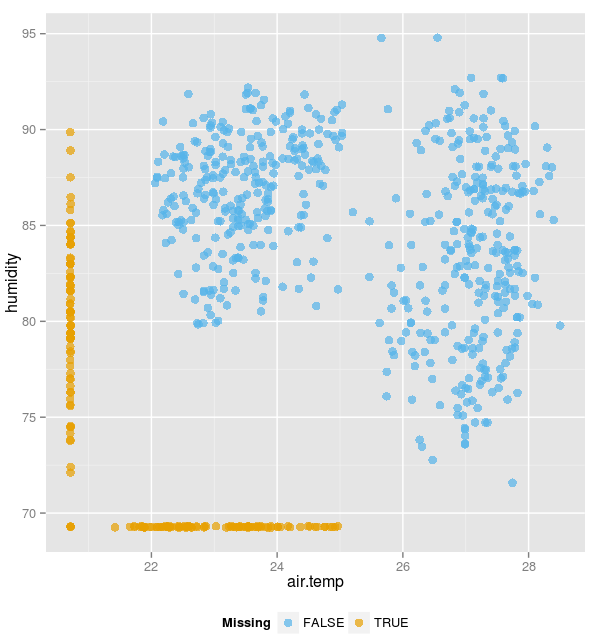
\includegraphics[width=0.31\textwidth]{graph/fig3-1-below10} &  &  & 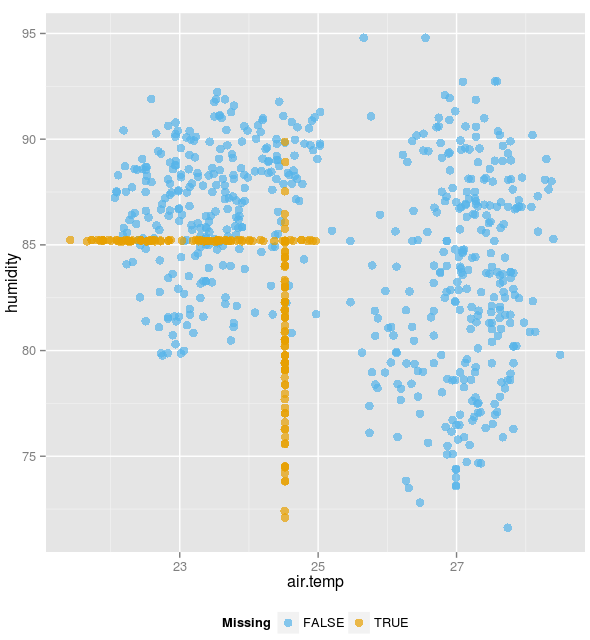
\includegraphics[width=0.31\textwidth]{graph/fig3-2-median}\tabularnewline
{\tiny{(c) Overall mean}} &  &  & {\tiny{(d) Random value}}\tabularnewline
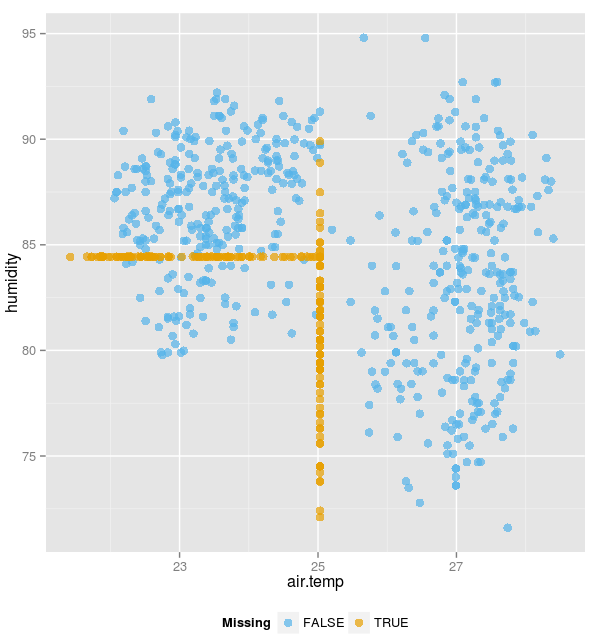
\includegraphics[width=0.31\textwidth]{graph/fig3-3-mean} &  &  & 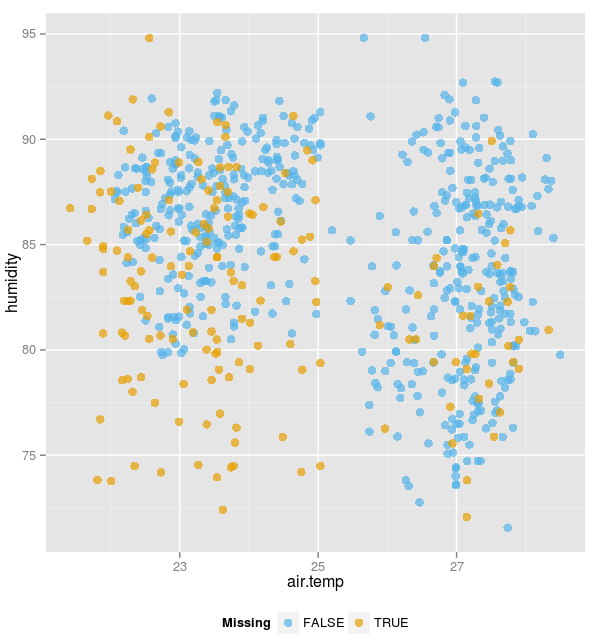
\includegraphics[width=0.31\textwidth]{graph/fig3-4-random}\tabularnewline
\end{tabular}
\par\end{centering}
\caption{Four panels of scatterplots displaying the results of different univariate imputations: (a) 10\% below the minimum (not strictly an imputation method, it is used for displaying missings as part of a plot of complete cases); (b) median of each variable; (c) mean of each variable; (d) random selection from the existing values.}
\label{fig:univariate-imputation}
\end{figure}
\par\end{center}

These imputation methods operate separately on each variable.  Dependencies between variables are ignored, yielding covariance and correlation estimates that are potentially very different from those of the complete cases. This could be a big problem for some analyses. These methods are not ideal from a statistical perspective.  In some situations where the inadequate estimation of covariance does not affect results and conclusions they can provide a simple, few assumptions required, solution, but in most situations they are not advised. For the application here, we are primarily concerned about providing methods for analysts to explore the missing value structure, and the plots reveal quite clearly why these univariate imputation methods are inadequate. Figure \ref{fig:univariate-imputation} shows the ``cross structure" (orange) induced on the pattern of points by mean and median imputation, and makes it quite clear that the covariance estimates for the imputed data would not well match that of the complete cases. 

\subsubsection{Neighbor imputations}


The ``Neighbor'' methods replace a missing value with the mean or a random value of its $k$ nearest complete neighbors (Figure~\ref{fig:neighbor-imputation}). Distance between two observations is calculated using Euclidean distance on the standardized variables that have no missings. Figure~\ref{fig:neighbor-diagram} explains the procedure. Ties are not considered, and only the first $k$ entries are used. 


\begin{center}
\begin{figure}[h]
\begin{centering}
\begin{tabular}{cccc}
{\tiny{(a) Mean of the neighbors}} &  &  & {\tiny{(b) Random neighbor}}\tabularnewline
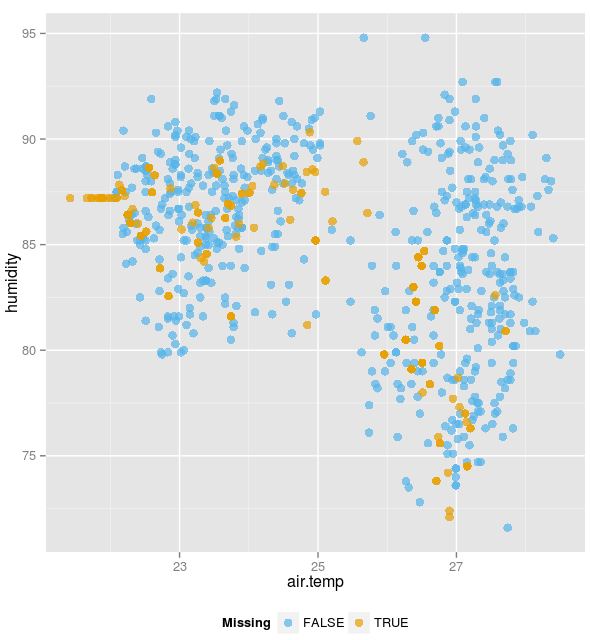
\includegraphics[width=0.32\textwidth]{graph/fig3-5-knn} &  &  & 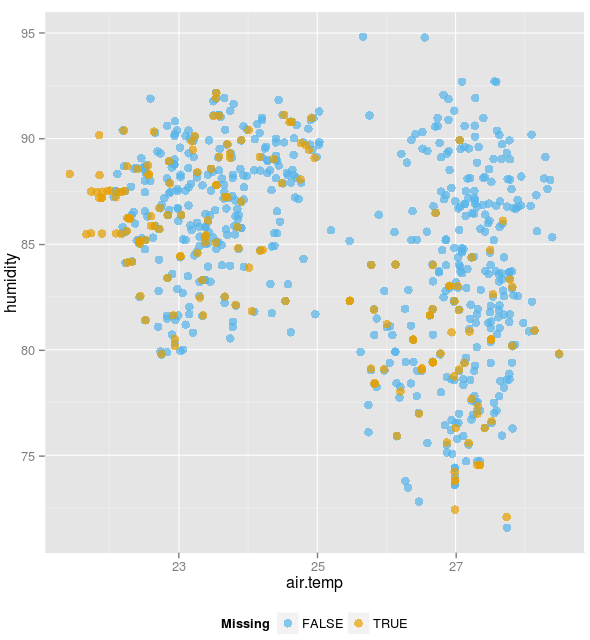
\includegraphics[width=0.32\textwidth]{graph/fig3-5-knn-2}\tabularnewline
\end{tabular}
\par\end{centering}
\caption{Scatterplots for two neighbor imputation methods: (a) mean of the 5 nearest neighbors, (b) a random value from the 5 nearest neighbors.}
\label{fig:neighbor-imputation}
\end{figure}
\par\end{center}


This method requires at least one case in the dataset to be complete, and no categorical variables can be used. (Ordinal variables are treated as integers.) If there are less than $k$ complete cases, then all of them are used to generate the mean or a random value. If none of the cases are complete, then the mean or a random value of the entire data will be returned. By default $k=5$, but the choice is changable.

%The methods should work well when the set of complete observations is large, but when there are few fully observations, the imputation may be biased due to too much waste information. 

The neighbor methods in \pkg{MissingDataGUI} can be seen as two special cases of hot deck imputation \citep{andridge2010review}. The neighbor mean method averages the weights on all chosen neighbors, and the random neighbor method places all the weights on one arbitrary neighbor. When $k=1$, the methods are deterministic hot deck.

\begin{center}
\begin{figure}[h]
\begin{centering}
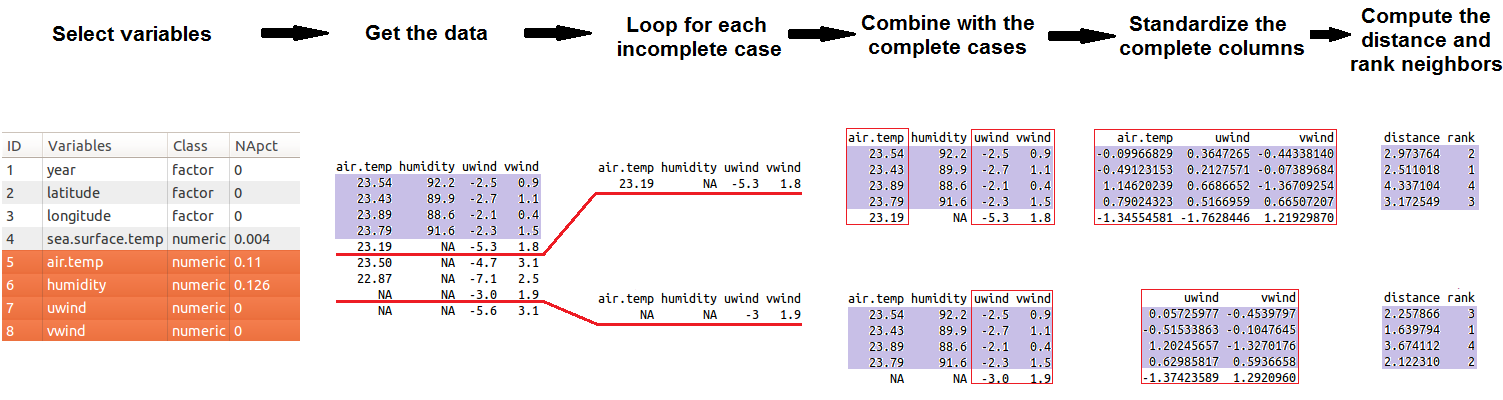
\includegraphics[width=1\textwidth]{graph/fig9-diagram}
\par\end{centering}
\caption{Illustration of the way to get $k$ nearest neighbors. The shaded entries are the complete observations to rank. The red frames circle the variables to compute the distance. After getting the rank of all complete observations, the first $k$ are used as neighbors. }
\label{fig:neighbor-diagram}
\end{figure}
\par\end{center}


\begin{center}
\begin{figure}[h]
\begin{centering}
\begin{tabular}{cccc}
{\tiny{(a) \pkg{Hmisc}: predictive mean matching}} &  &  & {\tiny{(b) \pkg{norm}: multivariate normal model}}\tabularnewline
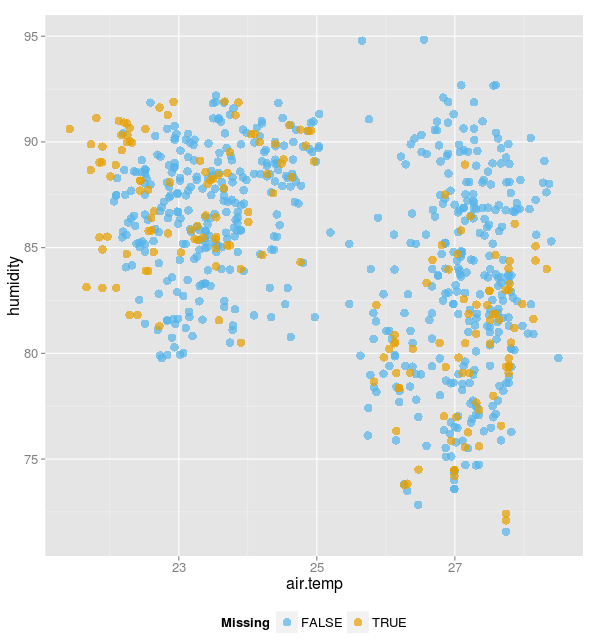
\includegraphics[width=0.32\textwidth]{graph/fig3-6-areg-2} &  &  & 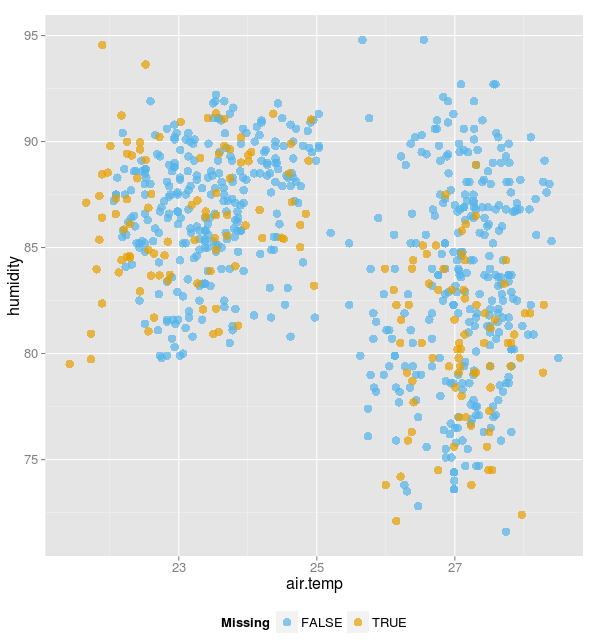
\includegraphics[width=0.32\textwidth]{graph/fig3-7-norm-2}\tabularnewline
{\tiny{(c) \pkg{mice}: chained equations}} &  &  & {\tiny{(d) \pkg{mi}: iterative regression}}\tabularnewline
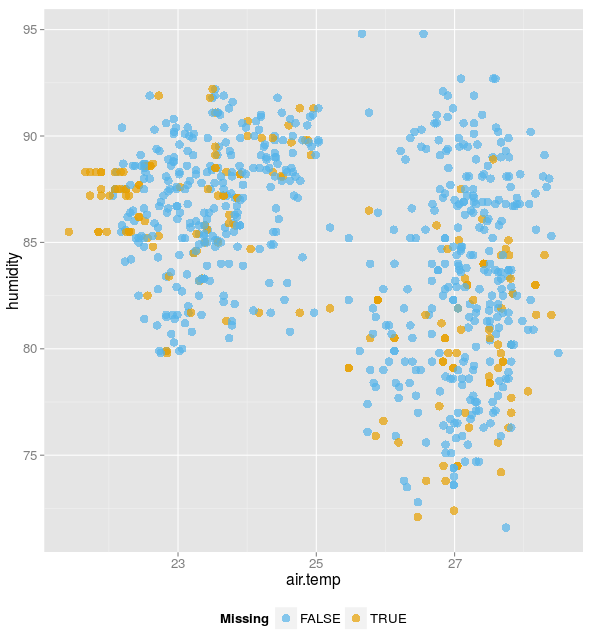
\includegraphics[width=0.32\textwidth]{graph/fig3-8-mice-2} &  &  & 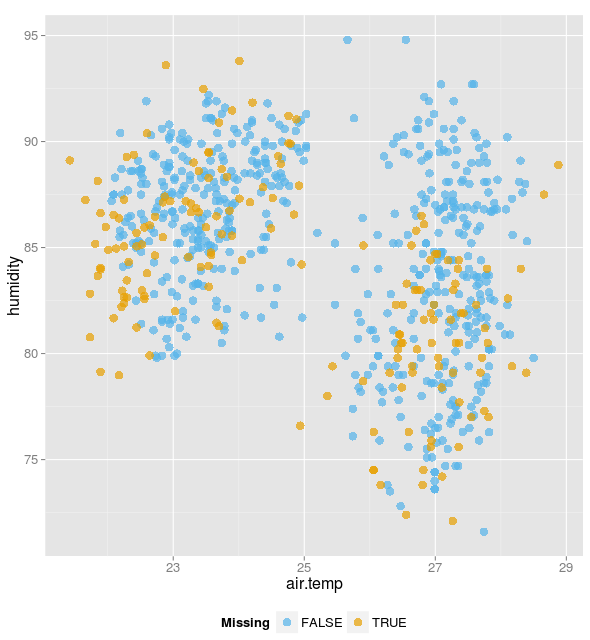
\includegraphics[width=0.32\textwidth]{graph/fig3-9-mi-2}\tabularnewline
\end{tabular}
\par\end{centering}
\caption{Scatterplots for the multiple imputations from four \proglang{R} packages: (a) predictive mean matching by \pkg{Hmisc}; (b) multivariate normal model by \pkg{norm}; (c) multivariate imputation by chained equations by \pkg{mice}; (d) multiple iterative regression imputation by \pkg{mi}. All the four imputations are conditioned on year.}
\label{fig:multiple-imputation}
\end{figure}
\par\end{center}

\clearpage
\subsubsection{Multiple imputations}

Multiple imputation, first proposed by \citet{rubin1978multiple}, is a method to get valid inferences by simulation. Multiple imputed datasets are generated based on the joint distribution and serve a wide variety of analytical goals. Four \proglang{R} packages are utilized to implement multiple imputations in the missing data GUI. Figure~\ref{fig:multiple-imputation} demonstrates the results of four packages on the same data. 

Among these packages, \pkg{norm} is quite different from the other three. \citet{schafer1998multiple} introduced the basic idea of \pkg{norm}. It assumes the observations are sampled from a multivariate normal distribution, and uses the EM algorithm to estimate the mean and variance-covariance matrix. It utilizes a data augmentation method to converge the distribution. 

All the other three packages are using a chained equation approach with similar steps but different settings. A comparison between the three packages is given in Table~\ref{tab:compare-mi}, based on \citet{hmisc}, \citet{mice}, and \citet{mi}. The main differences are that \pkg{Hmisc} provides three models with flexible drawing methods around the predicted values, and applies bootstrap to obtain a sample for every iteration. \pkg{mi} uses a convergence criterion to stop the iteration with some allowance for special situations. \pkg{mice} stands in the middle of the other two: the models provided are more flexible than \pkg{Hmisc}, but not as bayesian as \pkg{mi}.


\begin{center}
\begin{table}[h]
\begin{centering}
\begin{tabular}{l|c|c|c}
\hline 
\textbf{\scriptsize{Algorithm Steps}} & \textbf{\scriptsize{Hmisc}} & \textbf{\scriptsize{mice}} & \textbf{\scriptsize{mi}}\tabularnewline
\hline 
\textbf{\scriptsize{1. fill in the missing}} & \multicolumn{3}{c}{{\scriptsize{at random}}}\tabularnewline
\hline 
\textbf{\scriptsize{2. specify the model}} & {\scriptsize{pmm/regression/normpmm}} & \multicolumn{2}{c}{{\scriptsize{selectable model or user-specific model}}}\tabularnewline
\hline 
\textbf{\scriptsize{~~~~(default model)}} & \multicolumn{2}{c|}{{\scriptsize{predictive mean matching}}} & {\scriptsize{Baysian generalized linear models}}\tabularnewline
\hline 
\textbf{\scriptsize{3. decide the data}} & {\scriptsize{a bootstrap sample}} & \multicolumn{2}{c}{{\scriptsize{the entire dataset with the current imputed values}}}\tabularnewline
\hline 
\textbf{\scriptsize{4. iterate imputation}} & \multicolumn{3}{c}{{\scriptsize{in every cycle, variables with missings are imputed sequentially}}}\tabularnewline
\hline 
\textbf{\scriptsize{5. stop when}} & \multicolumn{2}{c|}{{\scriptsize{achieving the max \# of iterations}}} & {\scriptsize{difference of within and between variance is small}}\tabularnewline
\hline 
\end{tabular}
\par\end{centering}
\caption{Comparison of the algorithm steps among three multiple imputation packages that use chained equation approach.}
\label{tab:compare-mi}
\end{table}
\par\end{center}


By default, $m=3$ chains are imputed and users can modify the number of chains. Each chain will produce a result shown in a separate graphical panel. Switching among the panels the user can compare the results and observe discrepances. Figure~\ref{fig:chaintabs} shows the results of four different chains produced by \pkg{mice}. Three of the four produced results where a small dump of imputed values occurred.


\begin{center}
\begin{figure}[h]
\begin{centering}
\begin{tabular}{cccc}
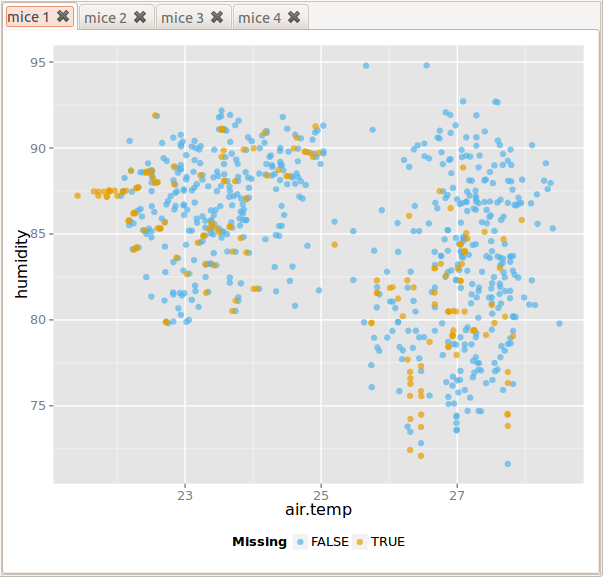
\includegraphics[width=0.4\textwidth]{graph/fig10-1-chain} &  &  & 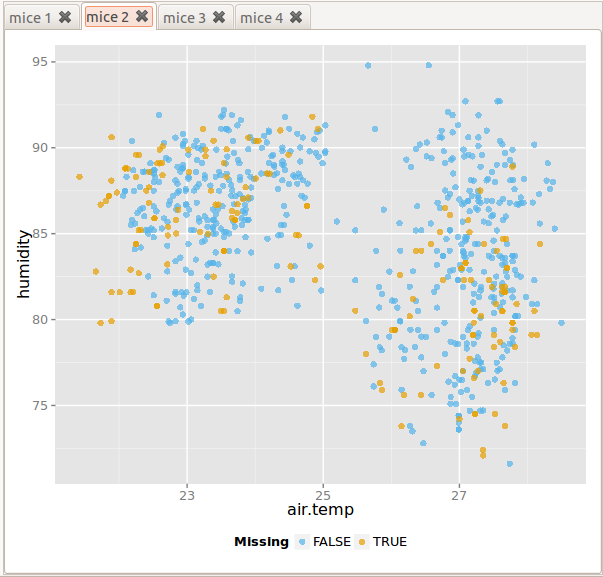
\includegraphics[width=0.4\textwidth]{graph/fig10-2-chain}\tabularnewline
%& & & \tabularnewline
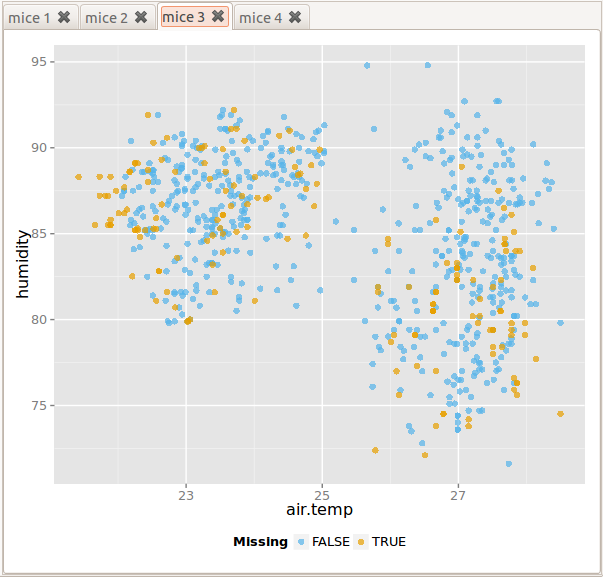
\includegraphics[width=0.4\textwidth]{graph/fig10-3-chain} &  &  & 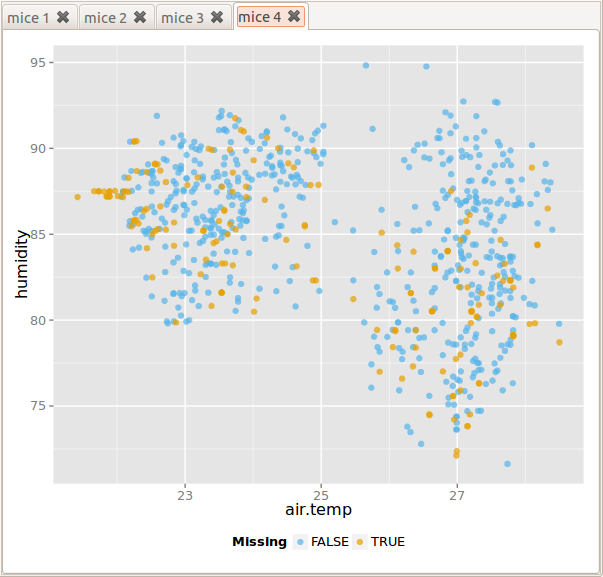
\includegraphics[width=0.4\textwidth]{graph/fig10-4-chain}\tabularnewline
\end{tabular}
\par\end{centering}
\caption{Results of four imputing chains by \pkg{mice}, starting with the default random seed. Users can switch the panels by clicking the tabs, or close a panel by hitting the `x' sign. Focusing on the imputed values when air temperatures around 22 degree, we see that the first, third and fourth chains cluster values in a small range of y-axis, but the second chain spread them very evenly in the y-direction.}
\label{fig:chaintabs}
\end{figure}
\par\end{center}


\subsubsection{Conditional on the categorical variables}

When the variables of interest are bimodal or multi-modal, using the center statistics like the mean or median for imputation, or the simulating from an overall estimate like \pkg{norm} does, is inadequate because the center does not reflect the shape of distribution properly. In many situations, the modalities arise from the mixture of groups. Hence, a better imputation method is to use the group means or medians instead of the overall mean or median.

This is available using the controls ``categorical variables to condition on''. All categorical variables are listed with checkboxes. The variables checked will partition the data into blocks and then the imputation method is implemented in each block of the data. However, the condition is invalid when the imputation method is ``Below 10\%'', since the aim of ``Below 10\%'' is only displaying the missings away from the non-missings. If the conditioning factor variable has missing values, then a ``factor = NA'' group will be generated to calculate the numeric summary or the imputed values. If the conditioning factor itself is one of the plotting variables, then a message box will emerge to ask the user to impute the factor before other variables, and the plots are created without the condition.

The role of conditioning in the imputation is revealed in Figure~\ref{fig: condition}. Without the condition, the imputations may locate far away from the distribution of values (Figure~\ref{fig: condition} left). But calculating separately by group provides a better result (Figure~\ref{fig: condition} right).


\subsection{Plot types}\label{plottype}

There are four types of graphs available in the missing data GUI: histogram (for continuous data)/ barchart (for categorical data), spinogram/spineplot, pairwise plots, and parallel coordinates plot. Figure~\ref{fig:graphtypes} displays all the graph types. Two color-blind friendly colors represent the observations and imputed values on any chosen variables. In Figure~\ref{fig:graphtypes} the yellow color means that the value is originally missing in humidity.


\begin{center}
\begin{figure}[h]
\begin{centering}
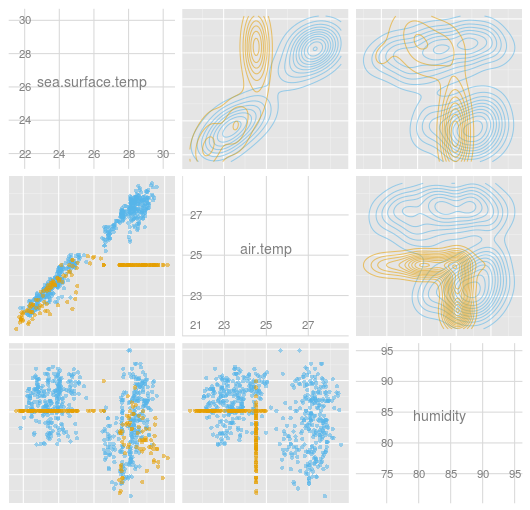
\includegraphics[width=.48\textwidth]{graph/fig4-1-median-uncondition}
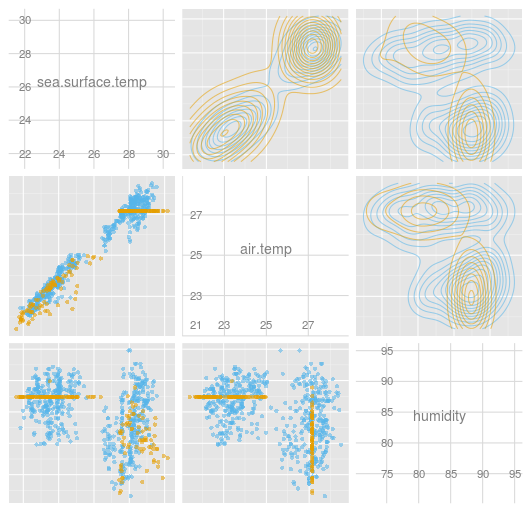
\includegraphics[width=.48\textwidth]{graph/fig4-2-median-condition}
\par\end{centering}
\caption{Comparison between imputations with and without conditions. The left panel is the imputation by median without condition and the right one is conditioned on year. In the left plot we can see that the imputed values fall between the two clusters, at the overall median. But when the imputation is conditioned on year (right plot), the imputed values are now better placed into the two clusters in the data.}
\label{fig: condition}
\end{figure}
\par\end{center}


\begin{center}
\begin{figure}[h]
\begin{centering}
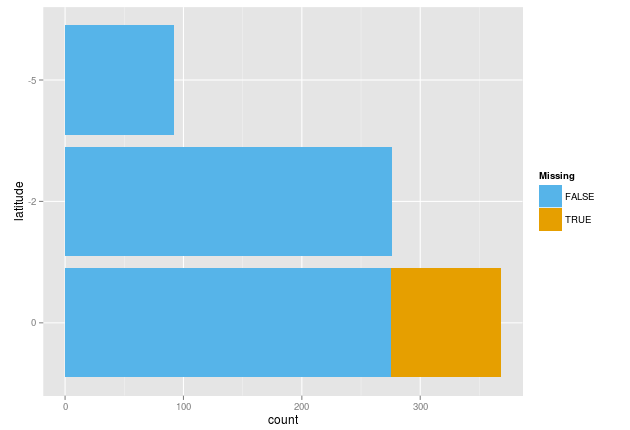
\includegraphics[width=.24\textwidth]{graph/fig5-1-barchart}
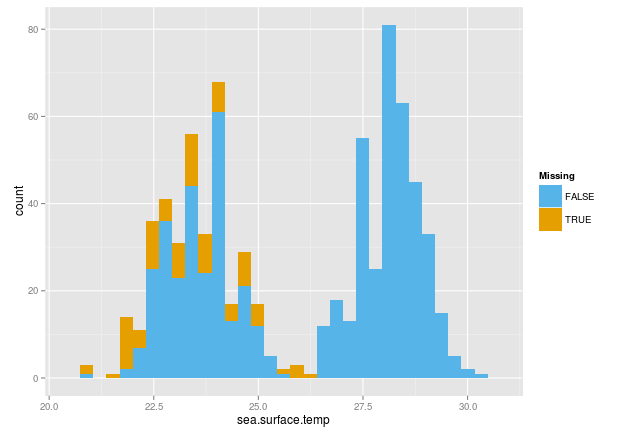
\includegraphics[width=.24\textwidth]{graph/fig5-1-histogram}
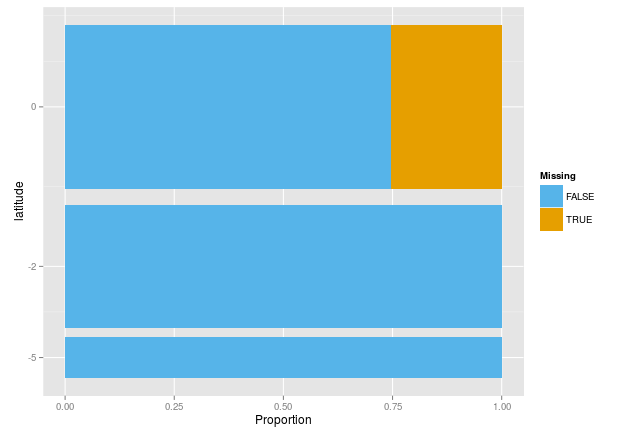
\includegraphics[width=.24\textwidth]{graph/fig5-1-spineplot-1}
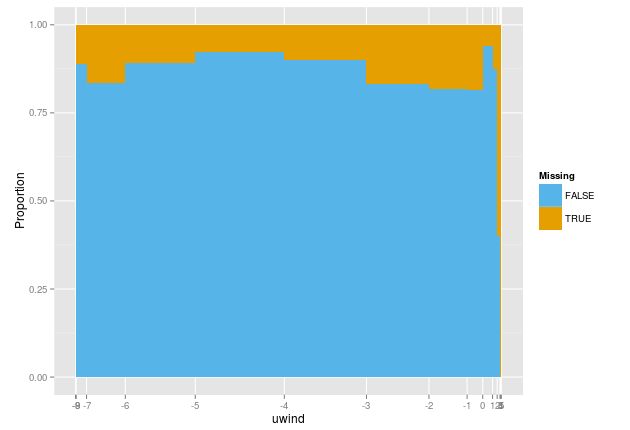
\includegraphics[width=.24\textwidth]{graph/fig5-1-spinogram-1}
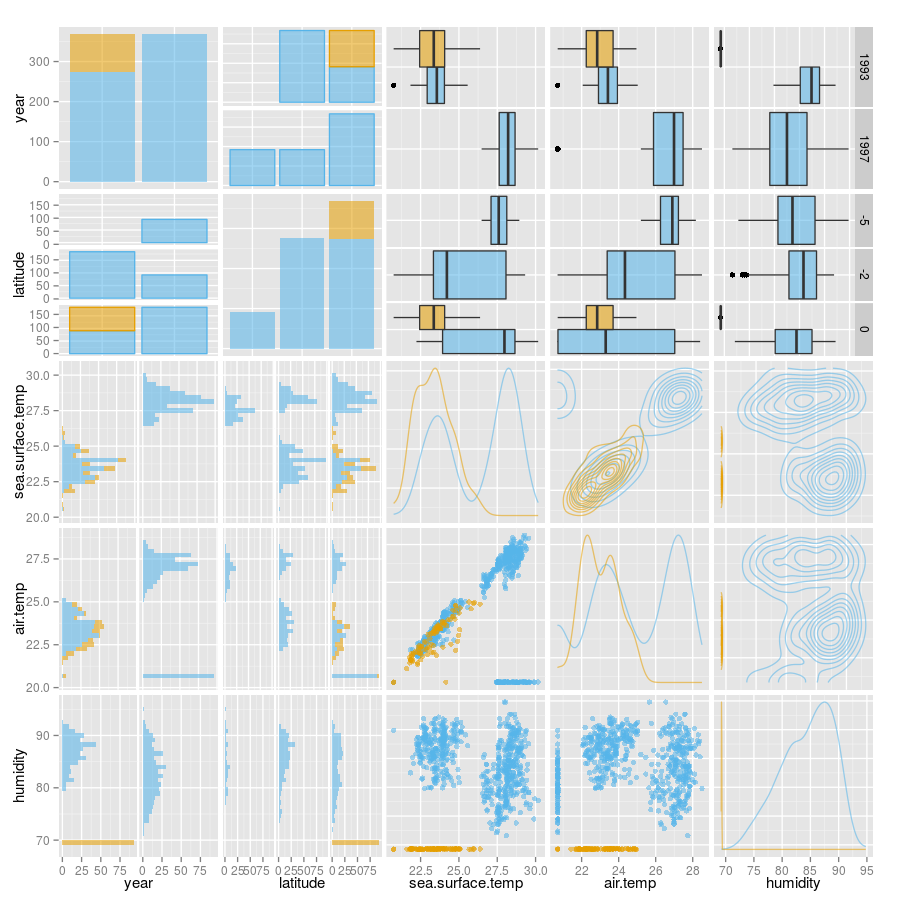
\includegraphics[width=.48\textwidth]{graph/fig5-2-pairwise}
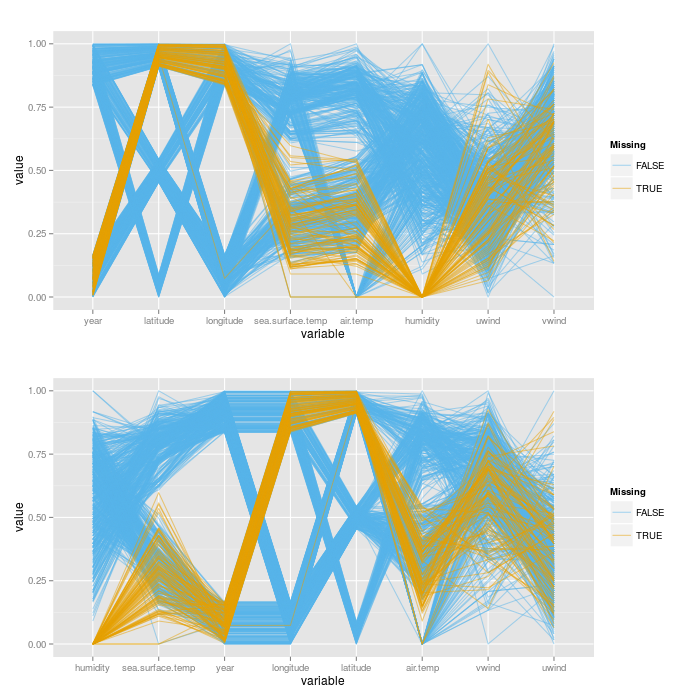
\includegraphics[width=.48\textwidth]{graph/fig5-2-pcp}
\par\end{centering}
\caption{Four types of graphs.
The first row from left to right are barchart, histogram, spineplot, and spinogram. The left panel on the second row are the pairwise plots, and the right shows two parallel coordinates plots. The order of variables is original on the upper plot, and on the lower one the variables separate the missing group and the complete group from the best to the worst. All the plots use ``below 10\%'' imputation and color by the missing of one variable - humidity.}
\label{fig:graphtypes}
\end{figure}
\par\end{center}


Histograms and barcharts are shown one by one for all the variables selected. When the missing values and the complete values share one bar, the bar is cut into two parts, and the ratio of two heights is equal to the ratio of missing and non-missing values in that bar.

The spinogram (for continuous variable) and spineplot (for categorical variable), introduced by \citet{hummel1996linked} and \citet{theus1999visualizing}, use width of the rectangle to represent count. Height is the same for all bars. The focus is on proportion for each group. The bars in the spinogram or spineplot are partitioned into two colors for the missing and non-missing values.

A scatterplot matrix is used to display pairs of variables. Variable names and scales are placed on the diagonal. For the continuous variables, the pairwise scatterplots are placed in the lower triangle, and the contour plots are shown in the upper triangle. For the categorical variables, barcharts by the categories of the vertical variable are given on both triangles. Again, the bars are colored in proportion to the missings. The combination of continuous and categorical variables is displayed as side-by-side boxplots of missing and non-missing values for each category on the upper triangle and side-by-side histograms on the lower triangle. Limited space available to the graphics device limits the number of variables that can be shown. The upper limit of the number of variables is set to be 5 and the lower limit is 2.

The parallel coordinates plot by \citet{inselberg1985plane} and \citet{wegman1990hyperdimensional} visualizes high-dimensional data. Though many plot types, like the scatterplot or histogram, are helpful to reveal the missing pattern, they are not convenient to display many variables simultaneously. Parallel coordinates plot, conversely, can give an overview on a relatively large quantity of variables. In the missing data GUI, the order of the variables can be chosen in one of two ways: the original order in the data, or by sorting the variables from the best separator to the worst by F statistic from ANOVA. In Figure~\ref{fig:graphtypes}, the best separating variable for the missingness of humidity is humidity itself, because the ``below 10\%'' method makes a big gap between the missing and non-missing values. ``Below 10\%'' is not an ideal method for the ordered parallel coordinates plot. However, the plot is still useful: it reveals that the missingness of humidity occurred in one year and one location, when sea.surface.temp and air.temp were low.


\subsection{Design issues}
%\subsection{Maps to items in GUIs}

The missing data GUI is designed in one window and three tabs. As shown in Figure~\ref{fig:missingGUI}, the summary tab includes all the important widgets: list of variables, radio for imputation methods, checkboxes for the conditional variables, the graphics device, etc.. An appropriate layout makes the widgets less crowded, and is easy to maintain. The other two tabs are not as critical as the main tab, but also play important roles.

The help tab shown in Figure~\ref{fig: missingGUI-tabs} (left) has the same layout as the summary tab. The only difference is that the graphics device is replaced by the help document. The corresponding help shows up when the user moves the mouse upon a widget.

The Settings tab shown in Figure~\ref{fig: missingGUI-tabs} (right) allows 
the user to choose options for the imputation methods in the 
package \pkg{mice}, as well as other settings for the multiple 
imputation, neighbor selection, and the display of parallel 
coordinates plot. To change the imputation models, users can double click a 
variable in the left table, and select any method provided in the pop-up window. 
The choices vary depending on the type of the variable.


%\begin{center}
\begin{figure}[h]
\begin{centering}
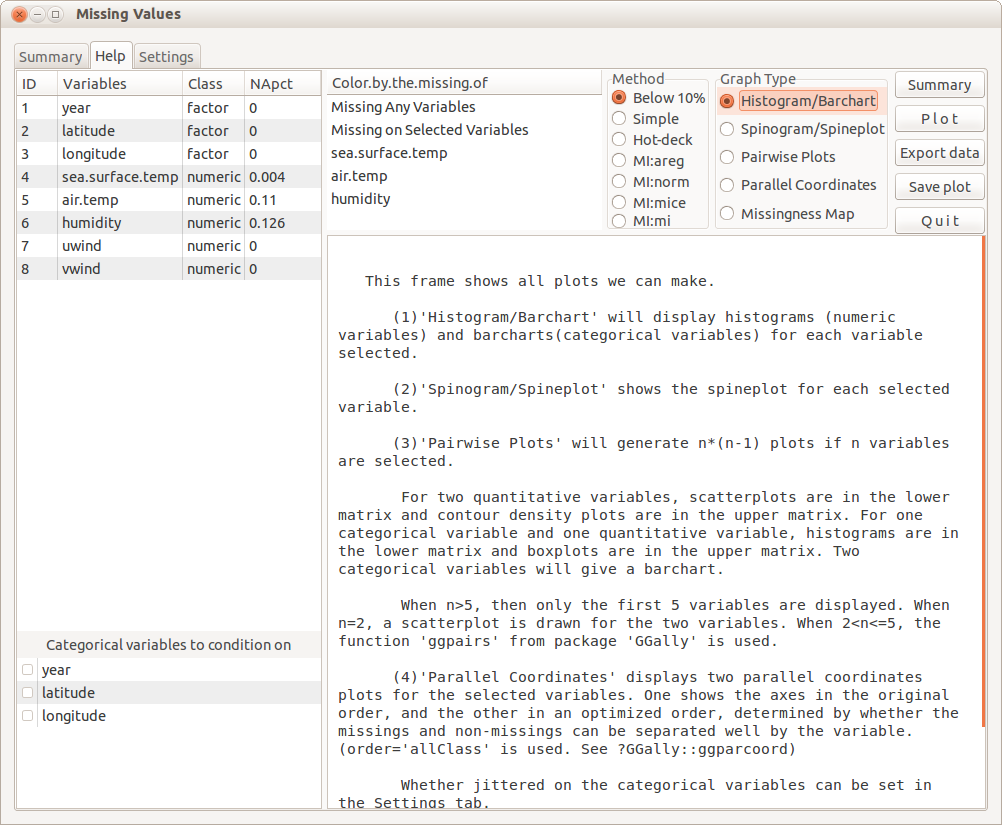
\includegraphics[width=0.49\textwidth]{graph/fig1-GUI-tab2} 
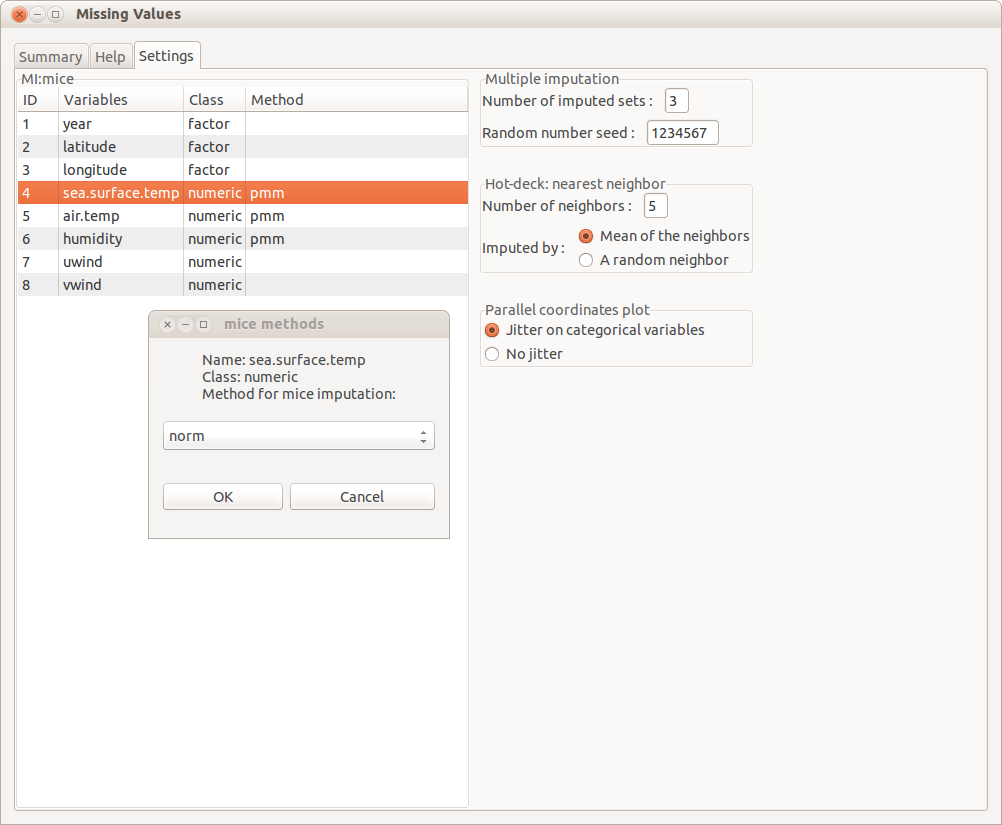
\includegraphics[width=0.49\textwidth]{graph/fig1-GUI-tab3}
\par\end{centering}
\caption{(Left) The help tab of the missing data GUI. Mousing over any part of the GUI or clicking the radio/checkbox items will pop up text explanations in the summary region. All the widgets have their detailed introduction. (Right) The Settings tab. Variables are listed with their classes in the left table. The fourth column gives the current \pkg{mice} methods for all incomplete variables. On the right, users can modify the number of imputed sets, random number seed, the number of neighbors, and the jitter setting for parallel coordinates plot.}
\label{fig: missingGUI-tabs}
\end{figure}
%\par\end{center}


\subsection{Data input and output}

Data can be read in as either a data frame or a comma separated values (csv) file. The preferred approach is to read an existing data frame in \proglang{R} because the type of variables (factor, numeric, ...) are preserved. \code{MissingDataGUI(data)} is the starting function in this case.

Reading from a csv file is another choice.  If \code{MissingDataGUI()} is called without a data frame argument, data import GUI is called (Figure~\ref{fig: import}). The ``Open'' button is for choosing files and the ``Watch Missing Values'' buttons will launch the missing data GUI. The file format must be csv currently, and only one data set can be imported every time, though more than one file can be opened in the data import GUI.

The imputed data can be saved using the ``Export data'' button. Only the selected variables will be imputed, but users could choose whether to export the selected columns or all the columns (with \code{NA}'s existing in the unselected variables). The shadow matrix is exported by default, so that analysts can always track back to find the locations of the real missings. As seen in Figure~\ref{fig: export}, data can be saved in three ways: csv file, rda file, or a data frame. The multiple imputed data from several chains will be saved as a list in rda format or data frame, and in seperate csv files otherwise.

The exported data with its shadow matrix can be loaded back again to the GUI, which implies the imputed data from other imputation methods (not provided by the missing data GUI) can also be imported. Users only need to provide a shadow matrix which indicates the locations of missings. In other words, the imported structure should be a data frame or a csv file with the first $n$ columns being the imputed data and the next $n$ columns being the shadow matrix.


\begin{center}
\begin{figure}[h]
\begin{centering}
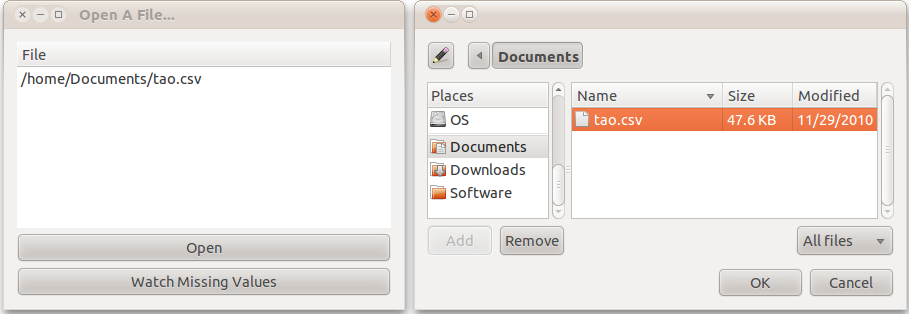
\includegraphics[width=0.8\textwidth]{graph/fig6-open}
\par\end{centering}
\caption{The data import GUI, with file selector, which is called by the ``open'' button. More than one file could be listed in the GUI, but only one data set is allowed active. The first file is automatically imported if none of the data sets are chosen when the ``Watching Missing Values'' button is hit.}
\label{fig: import}
\end{figure}
\par\end{center}


\begin{center}
\begin{figure}[h]
\begin{centering}
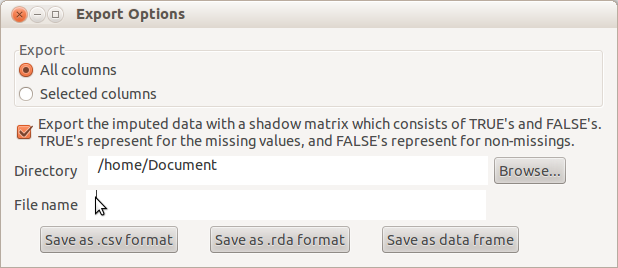
\includegraphics[width=0.6\textwidth]{graph/fig7-export}
\par\end{centering}
\caption{The data export GUI. By default, all columns are exported with a shadow matrix. The current working directory is set to be the default. Three exporting formats are provided.}
\label{fig: export}
\end{figure}
\par\end{center}


\subsection{Additional features of the GUI}

\begin{itemize}
\item Change the variable attributes. Double clicking on any variables in the top left table of the summary tab will open an attribute window, as displayed in Figure~\ref{fig: attributes}. Users could edit the variable name, or assign another class to the variable. When the class of a variable is switched from numeric/integer to character/factor/ordinal, the variable will be automatically loaded into the checkbox group as the potential conditioning variable.

\begin{center}
\begin{figure}[h]
\begin{centering}
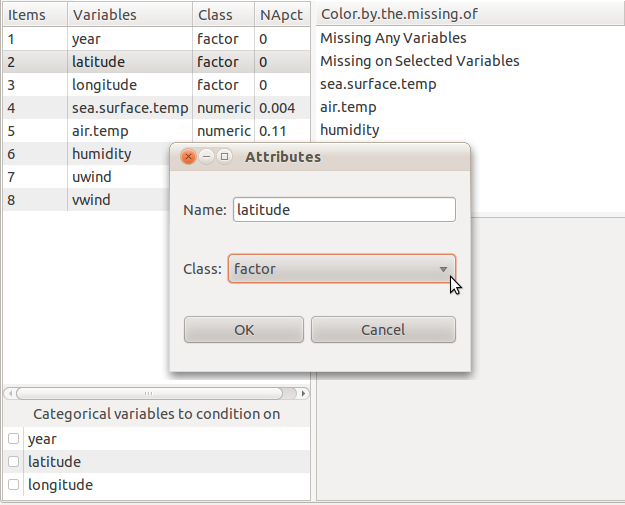
\includegraphics[width=0.6\textwidth]{graph/fig8-query}
\par\end{centering}
\caption{The attributes list for variable selection is interactive. The name can be edited, and the class could be changed to one of the five classes: integer, numeric, character, factor, or ordinal (factor). When a numeric variable is changed to a categorical variable, the widget for conditions will be updated.}
\label{fig: attributes}
\end{figure}
\par\end{center}

\item Search a variable by typing. The variable table, conditioning checkboxes, and color-by-variable selector allow text entry to find a variable. This feature is especially useful when there are many variables in the data.
\item Save the plots. Plots can be saved to png formatted files by ``Save plot'' button. The imputation method and plot type will be auto-completed in the file name.
\end{itemize}


\section{Example}\label{Examples}

\subsection{Data}

Two data sets are provided with the package: \code{tao}, which is used as the example in this section, and \code{brfss}. The \code{brfss} data is a subset of the 2009 survey from the Behavioral Risk Factor Surveillance System, an ongoing data collection program designed to measure behavioral risk factors for the US adult population (18 years of age or older). The website for this program is \url{http://www.cdc.gov/BRFSS/index.htm}.

The data \code{tao} is from the Tropical Atmosphere Ocean project (TAO) \citep{tao}. The TAO array consists of approximately 70 moorings in the Tropical Pacific Ocean, telemetering oceanographic and meteorological data to shore in real-time via the Argos satellite system. A subset of data from 6 moorings in 1993 and 1997 is used for the example. The data has 8 variables (year, latitude, longitude, sea surface temperature, air temperature, humidity, uwind and vwind) and 736 observations. The numeric summary of the 8 variables is shown in Figure~\ref{fig: num-summry}. This subset is provided by \citet{CS07}. We can open the GUI by the following commands:

\begin{Code}
library("MissingDataGUI")
MissingDataGUI(tao)
\end{Code}


\subsection{Exploring missings}

Three of the 8 variables have missing values. First, let's look at the distribution of missings on these variables. Figure~\ref{fig:tao1} (left) shows the pairwise plots of three variables (sea.surface.temp, air.temp, and humidity) with any missing values colored in yellow. Cases which are missing on humidity have low values of sea and air temperature. This suggests the dependence between humidity missingness and the temperature variables. Imputation methods that incorporate this dependence may be preferable.

Figure~\ref{fig:tao1} (right) shows the data imputed with median values (yellow). This imputation imposes a cross structure on the data, which does not match the shape of the complete cases. For example, there is a line of imputed values in the plot of air temperature versus sea surface temperature which is far from the rest of the complete cases. Thus the imputation method does not work well for this data.


\begin{figure*}[htp]
\centerline{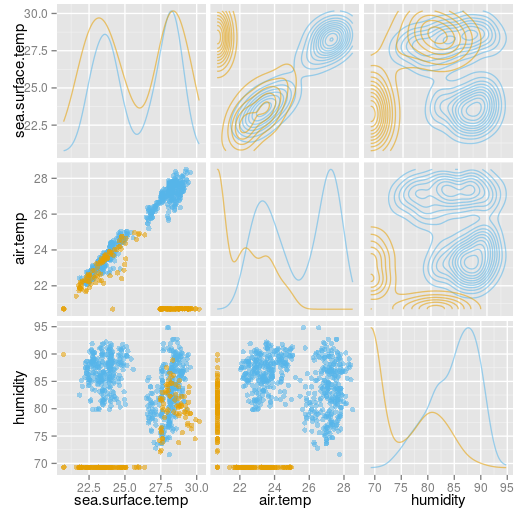
\includegraphics[width=0.49\textwidth]{graph/fig4-3-below10-uncondition}
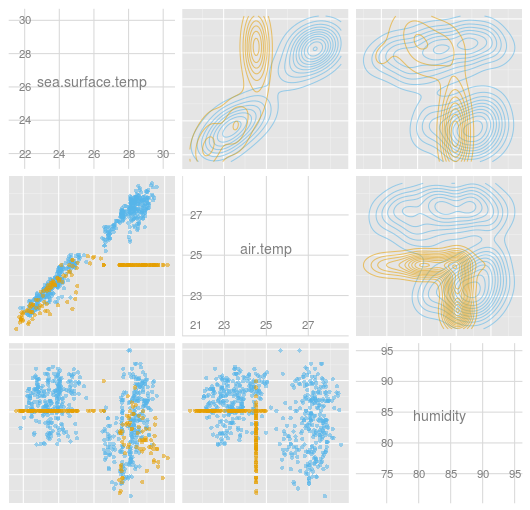
\includegraphics[width=0.49\textwidth]{graph/fig4-1-median-uncondition}}
\caption{(Left) Exploring the effect missingness on humidity, sea and air temperature. Missings on humidity (the bottom line of the third row) occur at the lower temperature values, suggesting a dependent relationship. Missing values are not missing completely at random. (Right) Exploring imputation methods. Imputation using the medians is shown here. Values that have been imputed are shown as yellow. Median imputation introduces a cross structure to the point scatter, and the imputed values don't match the data well, for example the line of imputed values is very apart from the complete cases in the plot of the tao temperature variables.}
\label{fig:tao1}
\end{figure*}


Figure~\ref{fig:tao3} (left) shows the data conditional imputing with median values (yellow) by year. This better matches the distribution of complete cases, although the imputed values still form bands in the scatterplot. This might be a problem because the variance estimation will be affected. 

For this data, the better ways to impute the data would take the strong association between the variables into account. This suggests that neighbor or multiple imputation might be the more desirable imputation methods. Figure~\ref{fig:tao3} (right) shows the results for MI:areg, the regression-based imputation, conditional on year. The imputed values match the distribution of complete cases reasonably well. There are a few slight concerns: some of the imputed values have lower air temperature values than any of the complete cases, the spread of the imputed values is a little greater than the complete cases. But overall, this is probably as good as it is going to get with imputing the missings for this data set. It would be reasonable to export the imputed data for further analysis at this point.


\begin{figure*}[htp]
\centerline{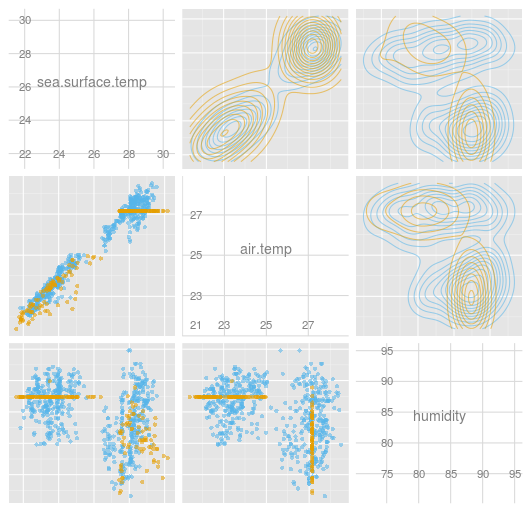
\includegraphics[width=0.49\textwidth]{graph/fig4-2-median-condition}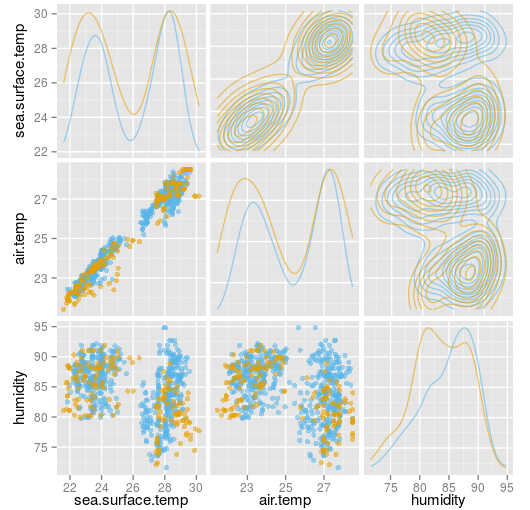
\includegraphics[width=0.49\textwidth]{graph/fig4-4-areg-condition}}
\caption{(Left) Imputation using the median conditional on year. Imputed values better match the complete cases, with the exception of the banding due to the fixed median value. (Right) Imputation using the multiple imputation MI:areg conditional on year. The distribution of imputed values is fairly close to the distribution of complete cases.}
\label{fig:tao3}
\end{figure*}


\subsection{Check assumptions}

In statistical methodology for imputation, there are three types of missing data mechanisms: MCAR (missing completely at random), MAR (missing at random), and MNAR (missing not at random). Many imputation methods, including multiple imputation, assume MCAR or MAR. However, MCAR is the most difficult mechanism to substantiate, because it requires that missingness be independent of the observed or other missing values. MAR is less strict, because it allows for kissings to be dependent on observed values, but it still expects the missingness to be independent from other missing values. To assess the adequacy of the assumptions, an important step is to review the data generation process. Beyond this we follow a process of elimination. The missing pattern is believed MCAR unless there is strong evidence against it. If MCAR is negated, then it is believed that the pattern is MAR, unless it is proven otherwise. If not MAR, then MNAR has to be assumed.

As an example, let us check whether the two incomplete variables (air.temp and humidity) in the data \code{tao} follows MCAR or MAR. Figure~\ref{fig:pcpCheck} gives two parallel coordinates plots, colored by the missingness of each incomplete variable. For example, the left panel is colored on the missingness of air.temp. Then the other 7 variables are given in the plot, and the yellow lines are the cases that are missing only on air.temp. The missing values on sea.surface.temp or humidity are represented by ``Below 10\%'' method. Most of the missings on air.temp occurred in one year and one location, with higher sea.surface.temp, higher uwind, and lower humidity. Most of the missings on humidity happened in the same location as the missings on air.temp but in another year, with lower sea.surface.temp and lower air.temp. This is strong evidence against MCAR.

\begin{center}
\begin{figure}[h]
\begin{centering}
\begin{tabular}{cc}
{\tiny{air.temp}} & {\tiny{humidity}}\tabularnewline
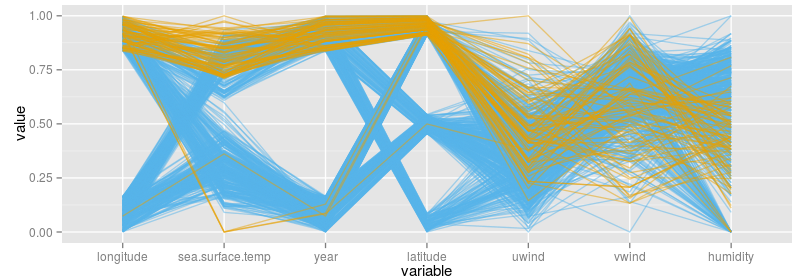
\includegraphics[width=.48\textwidth]{graph/fig12-2-air-temp-2} & 
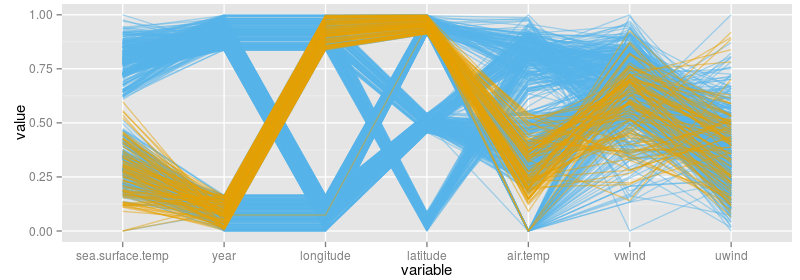
\includegraphics[width=.48\textwidth]{graph/fig12-3-humidity-2} \tabularnewline
\end{tabular}
\par\end{centering}
\caption{Parallel coordinates plots colored by whether missing on air.temp(left) or humidity(right). The variables are sorted by the F statistic of ANOVA, i.e., if the difference between the missing data and the observed data is significant. Any missing values in the present variables are imputed by ``Below 10\%'' method. Obviously the missingness on air.temp and humidity associates with other variables like year and location, so the MCAR assumption on these two variables are violated.}
\label{fig:pcpCheck}
\end{figure}
\par\end{center}


In general, we are not able to reject MAR from the plots, even when we see an obvious difference between missings and non-missings, since the real values of the missings are not available. For example, in Figure~\ref{fig:uvwind}, the distributions of uwind and vwind conditioned on the missingness of air.temp are different, since the missings on air.temp are higher in uwind and more scattered in vwind. The reasoning is complicated, but we cannot reject MAR. It is possible that, conditional on uwind and vwind, that the distribution of true air.temp values of the missings is the same as that of the observed values. Thus, uwind and vwind remove any dependence of missing status for the air.temp variable. Generally, it is not possible to establish MNAR without actually knowing the true values of the missings. However, for this data, the plots suggest that the imputation of air.temp should involve uwind and vwind.


\begin{center}
\begin{figure}[h]
\begin{centering}
\begin{tabular}{ccc}
{\tiny{Missing on air.temp}} && {\tiny{Missing on humidity}}\tabularnewline
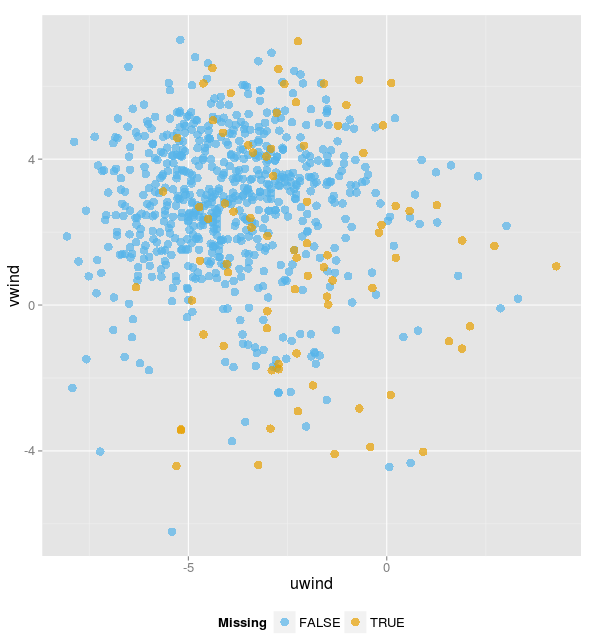
\includegraphics[width=.35\textwidth]{graph/fig11-1-air-temp} && 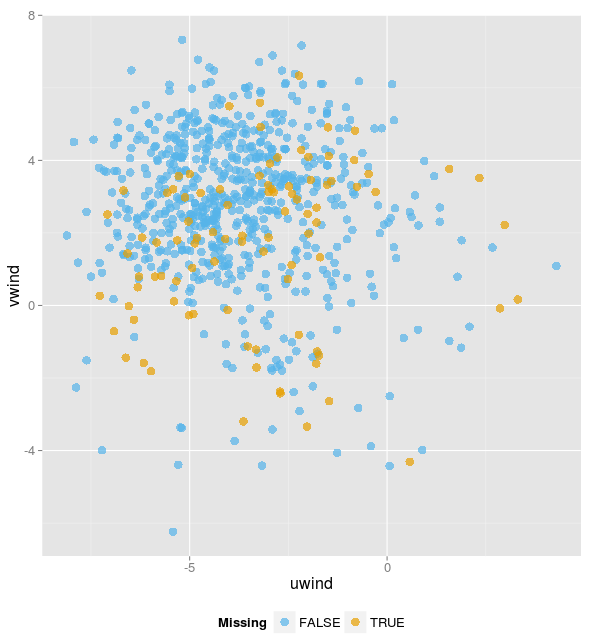
\includegraphics[width=.35\textwidth]{graph/fig11-3-humidity}\tabularnewline
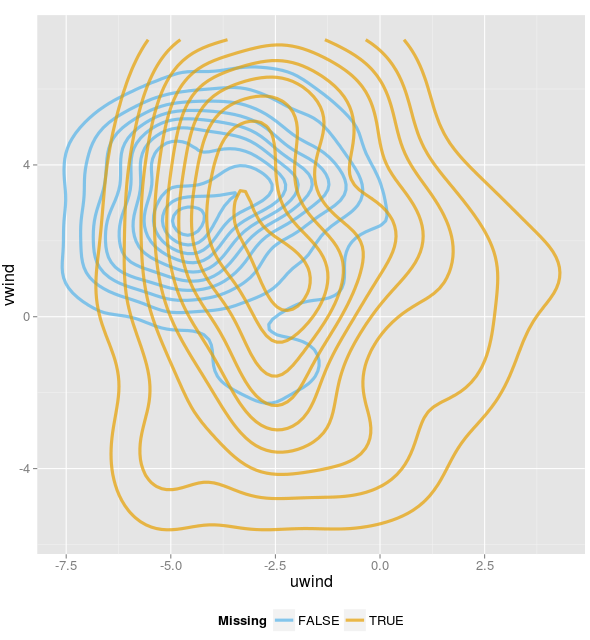
\includegraphics[width=.35\textwidth]{graph/fig11-2-air-temp} && 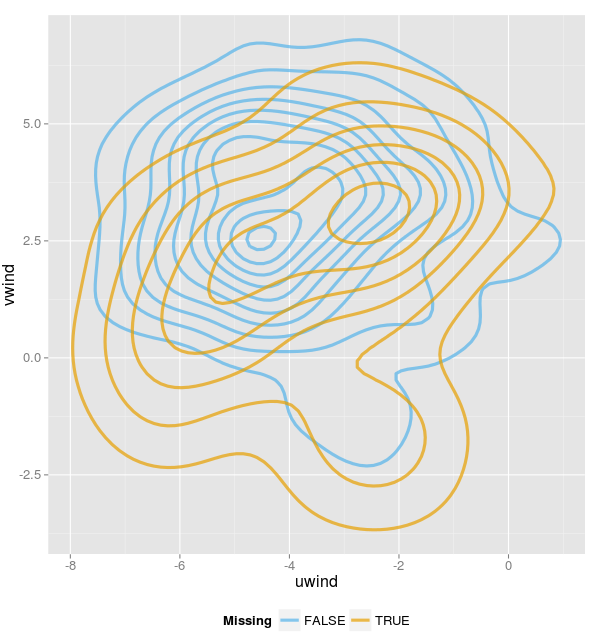
\includegraphics[width=.35\textwidth]{graph/fig11-4-humidity}\tabularnewline
\end{tabular}
\par\end{centering}
\caption{Scatterplots (top row) and contour plots (bottom row) of uwind and vwind, two complete variables, colored by whether missing on air.temp(left column) or humidity(right column). The missings of air.temp is averagely higher on uwind and has a larger variation, than the non-missings of air.temp. In reverse, the joint distribution of uwind and vwind on the missings of humidity is closer to that of the non-missings.}
\label{fig:uvwind}
\end{figure}
\par\end{center}


\section{Summary}

The MissingDataGUI  package makes it possible to explore patterns of missingness in data and the impact of various imputation methods on the distribution of values in the data. Future work would add interaction to the plots so that it is possible to brush points to more completely explore missing structure, as can be done in \proglang{GGobi} and \proglang{MANET}.


\section*{Software}

This missing data GUI is written in \proglang{R} 3.0.2 \citep{r} and based on the package \pkg{gWidgets} \citep{gwidgets} with the toolkit \proglang{RGtk2}. 

On different platforms (Windows, Linux, Mac) the appearance of the GUI will differ slightly, but the functionality will be the same.

The histogram/barchart, spinogram/spineplot, and missingness map are generated using \pkg{ggplot2} \citep{ggplot2}.
The scatterplot matrix and parallel coordinates plot are produced by package \pkg{GGally} \citep{ggally}.

\section*{Acknowledgements}

This work was partially supported by an unrestricted fellowship from Novartis, and National Science Research grant DMS0706949.

\bibliography{MissingDataGUI}
\end{document}
